\documentclass[11pt, psamsfonts,reqno]{amsart}
\usepackage{amssymb,amsfonts,amsmath,graphicx,lineno}
\usepackage[colorlinks=true, citecolor=cyan, urlcolor=black, linkcolor=red]{hyperref}
\usepackage{color}
\usepackage{tikz}
\usetikzlibrary{shapes, arrows}
\usepackage{pgfplots}
\tikzset{>= angle 60}
\usepackage{tikz-cd}
\usepackage{amsmath}
\usepackage{amssymb}
\usepackage{color}

\begin{document}

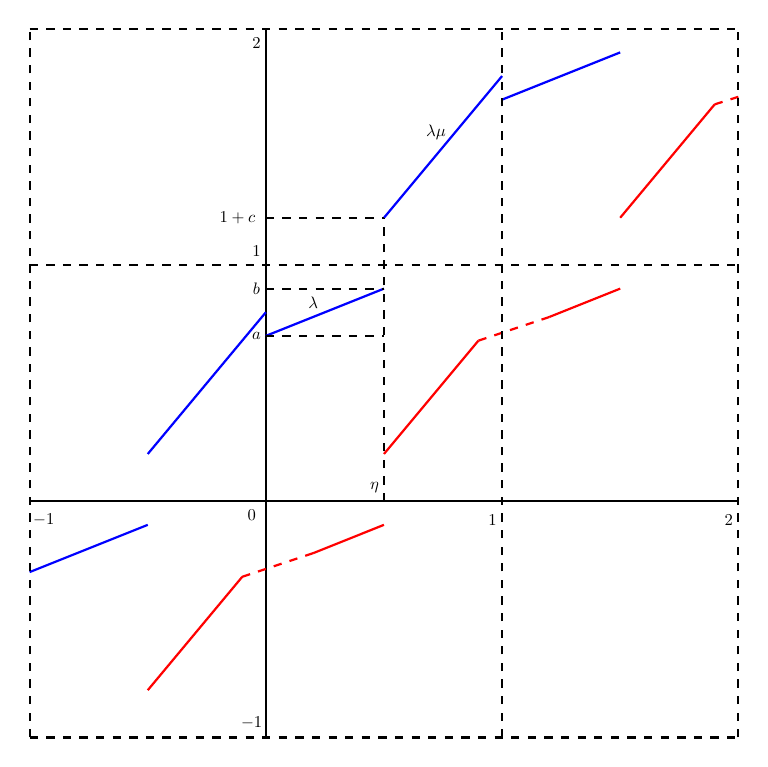
\begin{tikzpicture}[thick,scale=0.6, every node/.style={scale=0.6}]
\draw (-5,0) -- (10,0);
\draw (0,-5) -- (0,10);
\draw[dashed,red]   (-0.5,3.4-5) -- (1,3.9-5);
\draw[thick,red]  (-2.5,-4) -- (-0.5,3.4-5);
\draw[thick,red]   (1,3.9-5) -- (2.5,4.5-5);
\draw[dashed,red]   (-0.5+5,3.4-5+5) -- (1+5,3.9-5+5);
\draw[thick,red]  (-2.5+5,-4+5) -- (-0.5+5,3.4-5+5);
\draw[thick,red]   (1+5,3.9-5+5) -- (2.5+5,4.5-5+5);

\draw[dashed,red]   (9.5,8.4) -- (10,8.56);
\draw[thick,red]  (-2.5+5+5,-4+5+5) -- (-0.5+5+5,3.4-5+5+5);

\draw[thick,blue]   (0,3.5) -- (2.5,4.5);
\draw[thick,blue]   (-5,-1.5) -- (-2.5,-0.5);
\draw[thick,blue]   (5,8.5) -- (7.5,9.5);
\draw[thick,blue]  (2.5,6) -- (5,9);
\draw[thick,blue]  (-2.5,1) -- (0,4);
\node   at (-0.3,-0.3) {$0$};
\node   at (-0.3,-4.7) {$-1$};
\draw[dashed] (0,6) -- (2.5,6);
\draw[dashed] (-5,5) -- (10,5);
\draw[dashed] (-5,10) -- (10,10);
\draw[dashed] (-5,-5) -- (10,-5);
\draw[dashed] (5,-5) -- (5,10);
\draw[dashed] (-5,-5) -- (-5,10);
\draw[dashed] (10,-5) -- (10,10);
\draw[dashed] (0,4.5) -- (2.5,4.5);
\draw[dashed] (0,3.5) -- (2.5,3.5);
\node at (1,4.2) {$\lambda$};
\node at (3.6,7.8) {$\lambda\mu$};
\node at (-0.2,4.5) {$b$};
\node   at (-0.6,6) {$1+c$};
\node at (2.3,0.3) {$\eta$};
\node   at (-0.2,5.3) {$1$};
\node   at (-0.2,9.7) {$2$};
\node   at (-0.2,3.5) {$a$};
\node   at (4.8,-0.4) {$1$};
\node   at (9.8,-0.4) {$2$};
\node   at (-4.7,-0.4) {$-1$};
\draw[dashed]  (2.5,0) -- (2.5,6);
\end{tikzpicture}

\end{document}